\chapter{Описание продукта и принцип работы}\label{ch:description-ru}

\section{Назначение}
Приборные панели \ReplicaGenOne{} и \ReplicaNextLong{} заменяют штатные кластерные щитки Volkswagen и расширяют их функциональность.
Они обеспечивают цифровую индикацию скорости, оборотов двигателя, температуры охлаждающей жидкости, уровня топлива и вычислений MFA, а также поддерживают датчики скорости с тросовым и электронным приводом.
Модели \ReplicaGenOneShort{} оснащены встроенным Bluetooth-контроллером, а \ReplicaNextShort{} дополняются модулями конфигурации по Wi-Fi и опциональными блоками расширения.

\section{Идентификация моделей}
Каждый щиток маркируется четырёхбуквенным кодом, описывающим тип силовой установки, способ сборки, интерфейс датчика скорости и поколение жгута.
Дополнительные цифры указывают поддерживаемый диапазон тахометра, а трёхбуквенный суффикс отражает экспортные единицы измерения.

\subsection{Четырёхбуквенное обозначение}
\begin{description}
    \item[Позиция~1] \textbf{G} для бензиновых двигателей или \textbf{D} для дизельных.
    \item[Позиция~2] \textbf{A} для заводской сборки или \textbf{M} для наборов самостоятельной сборки.
    \item[Позиция~3] \textbf{C} для тросового датчика скорости или \textbf{R} для электронного датчика.
    \item[Позиция~4] \textbf{T} для жгута до рестайлинга (CE~1) или \textbf{S} для жгута после рестайлинга (CE~2).
\end{description}
Замыкающая цифра обозначает максимальные обороты двигателя на шкале тахометра в тысячах RPM (например, «8» в GACT8 соответствует шкале до 8000~об/мин).

\subsection{Суффикс единиц измерения}
Экспортные версии могут дополняться трёхбуквенным суффиксом из набора \texttt{MGFK}:
\begin{description}
    \item[M] мили в час,
    \item[G] галлоны,
    \item[F] градусы Фаренгейта,
    \item[K] градусы Кельвина.
\end{description}
Например, щиток \texttt{GART8-MGF} — это бензиновая, заводская, с электронным датчиком скорости и жгутом CE~2 приборка с тахометром на 8000~об/мин и имперскими единицами измерения.

\section{Линейка моделей}
{\scriptsize
\begin{tblr}{
    colspec={Q[l,2.2cm] X[l]},
    hlines
}
\textbf{Модель} & \textbf{Описание} \\
GACT & Бензин, заводская сборка, тросовый датчик скорости, два разъёма, шкала 7000~об/мин. \\
GART & Бензин, заводская сборка, внешний электронный датчик скорости, два разъёма, шкала 7000~об/мин. \\
GAC & Бензин, заводская сборка, тросовый датчик скорости, один разъём, шкала 7000~об/мин. \\
GARS & Бензин, заводская сборка, внешний электронный датчик скорости, один разъём, шкала 7000~об/мин. \\
GACT8 & Бензин, заводская сборка, тросовый датчик скорости, два разъёма, шкала 8000~об/мин. \\
GART8 & Бензин, заводская сборка, внешний электронный датчик скорости, два разъёма, шкала 8000~об/мин. \\
GACS8 & Бензин, заводская сборка, тросовый датчик скорости, один разъём, шкала 8000~об/мин. \\
GARS8 & Бензин, заводская сборка, внешний электронный датчик скорости, один разъём, шкала 8000~об/мин. \\
DACT & Дизель, заводская сборка, тросовый датчик скорости, два разъёма, шкала 6000~об/мин. \\
DART & Дизель, заводская сборка, внешний электронный датчик скорости, два разъёма, шкала 6000~об/мин. \\
DACS & Дизель, заводская сборка, тросовый датчик скорости, один разъём, шкала 6000~об/мин. \\
DARS & Дизель, заводская сборка, внешний электронный датчик скорости, один разъём, шкала 6000~об/мин. \\
MT & Набор для самостоятельной сборки с двумя разъёмами. \\
M.S. & Набор для самостоятельной сборки с одним разъёмом. \\
NEXT-GART & \ReplicaNextLong{}, шкала 8000~об/мин, два разъёма, электронный датчик скорости. \\
NEXT-GARS & \ReplicaNextLong{}, шкала 8000~об/мин, один разъём, электронный датчик скорости. \\
NEXT-MT & Набор \ReplicaNextLong{} для самостоятельной сборки с двумя разъёмами. \\
NEXT-MS & Набор \ReplicaNextLong{} для самостоятельной сборки с одним разъёмом. \\
\end{tblr}}

\section{Распиновка разъёмов}
\subsection{Щитки с двумя разъёмами}
\begin{figure}[htbp]
    \centering
    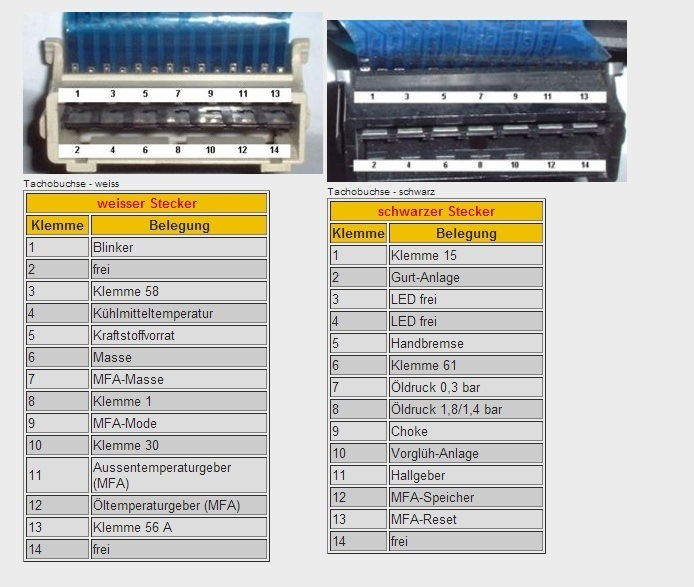
\includegraphics[width=0.72\textwidth]{digifiz_manual/image008.jpg}
    \caption{Схема разъёмов для приборных панелей \ReplicaGenOne{} с двумя колодками.}
\end{figure}

\noindent\textbf{Белый разъём}

{\scriptsize
\begin{tblr}{
    colspec={Q[l,1.4cm] X[l]},
    hlines
}
\textbf{Пин} & \textbf{Назначение} \\
1 & Выход указателя поворота, замкнут на массу для лампы индикатора. \\
2 & Frei — не подключён. \\
3 & Клемма~58, положительное питание подсветки панели. \\
4 & Вход резистивного датчика температуры охлаждающей жидкости. \\
5 & Вход резистивного датчика уровня топлива. \\
6 & Общая масса. \\
7 & Дополнительная масса. \\
8 & Сигнал оборотов двигателя с клеммы~1 (катушка, трамблёр или другая форма до 12~В с возможными импульсами до 300~В). \\
9 & Линия режимов MFA для переключения функций MFA. \\
10 & Постоянное питание UNR (не используется в \ReplicaGenOneShort{}, основное питание в \ReplicaNextShort{}). \\
11 & Провод «+» датчика наружной температуры MFA (\ReplicaNextShort{}). \\
12 & Провод датчика температуры масла MFA (только \ReplicaNextShort{}). \\
13 & Вход индикатора дальнего света KL~56a (активен при +12~В). \\
\end{tblr}}

\noindent\textbf{Чёрный разъём}

{\scriptsize
\begin{tblr}{
    colspec={Q[l,1.4cm] X[l]},
    hlines
}
\textbf{Пин} & \textbf{Назначение} \\
1 & Клемма~15, +12~В от замка зажигания. \\
2--4 & Не подключены. \\
5 & Вход индикатора стояночного тормоза (активен при подаче на массу). \\
6 & Выход лампы генератора KL~61 с возбуждающим резистором 120~\ensuremath{\Omega}. \\
7 & Датчик давления масла 0,3~бар. \\
8 & Датчик давления масла 1,8~бар. \\
9 & Не используется. \\
10 & Вход индикатора свечей накала (+12~В, только для дизеля). \\
11 & Вход датчика Холла для опциональных датчиков скорости. \\
12 & Линия выбора блока MFA. \\
13 & Линия сброса MFA. \\
\end{tblr}}

\subsection{Щитки с одним разъёмом}
Приборные панели с одним разъёмом используют разводку, показанную на \autoref{fig:single-connector}.
Жгут содержит те же сигналы, что и в двухразъёмных версиях, но объединяет их в один разъём.

\begin{figure}[htbp]
    \centering
    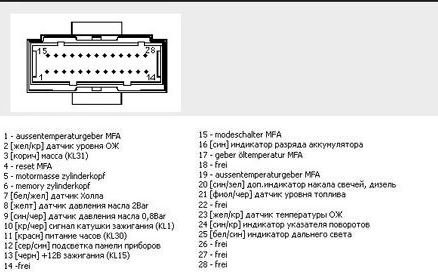
\includegraphics[width=0.65\textwidth]{digifiz_manual/image009.png}
    \caption{Схема одинарного разъёма, применяемого в компактных версиях Replica.}
    \label{fig:single-connector}
\end{figure}

\subsection{Предварительный жгут Scirocco/Passat}
Проектный жгут Scirocco/Passat использует два разъёма. Их функции сведены ниже.

\noindent\textbf{5-контактный разъём}
{\scriptsize
\begin{tblr}{
    colspec={Q[l,2.6cm] X[l]},
    hlines
}
\textbf{Пин} & \textbf{Назначение} \\
1~(D3) & Контакт индикатора диапазона «D» АКПП. Замыкает лампу «D» на массу при положении селектора~D. \\
2~(D2) & Контакт индикатора второго диапазона АКПП. Замыкает лампу «2» на массу при положении селектора~2. \\
3~(D1) & Контакт индикатора пониженного диапазона АКПП. Замыкает лампу «1» на массу при положении селектора~1. \\
4~(SA) & Общий плюс индикации селектора (\emph{Schaltanzeige}); обеспечивает питание +12~В для ламп диапазонов. \\
5~(SPERRE) & Контакт блокировки запуска от селектора. Замкнут в положениях P или N, позволяя запуск двигателя. \\
\end{tblr}}

\noindent\textbf{14-контактный разъём}
{\scriptsize
\begin{tblr}{
    colspec={Q[l,2.6cm] X[l]},
    hlines
}
\textbf{Пин} & \textbf{Назначение} \\
1~(KL~58) & Питание подсветки панели. \\
2~(MASS) & Возврат на массу. \\
3~(TANK) & Вход датчика уровня топлива. \\
4~(TEMP) & Вход датчика температуры охлаждающей жидкости. \\
5~(KL~1) & Сигнал оборотов двигателя (клемма~1). \\
6~(UHR) & Постоянный +12~В для часов и памяти. \\
7~(FERNL) & Вход индикатора дальнего света. \\
8~(reserved) & Не подключён. \\
9~(OEL~1.8) & Датчик высокого давления масла 1,8~бар. \\
10~(CAT~VORGL(-)) & Вход лампы предпускового подогрева/накала (активный низкий). \\
11~(OEL~0.3) & Датчик низкого давления масла 0,3~бар. \\
12~(KL~61) & Лампа генератора и цепь возбуждения. \\
13~(KL~49a) & Общий вход указателей поворота. \\
14~(KL~15) & Питание +12~В от зажигания. \\
\end{tblr}}

\subsection{Соответствие разъёмов Mk1}
В автомобилях Volkswagen Mk1 используются следующие назначения:
\begin{enumerate}
    \item Питание подсветки и ближнего света.
    \item Масса MASSE~31.
    \item Датчик уровня топлива TANK.
    \item Датчик температуры охлаждающей жидкости TEMP.
    \item Сигнал тахометра KL~1.
    \item Постоянное питание UHR.
    \item Сигнал дальнего света KL~56.
    \item Датчик высокого давления масла 1,8~бар.
    \item Датчик низкого давления масла 0,3~бар.
    \item Индикатор свечей накала дизеля.
    \item Вход CHOKE (не используется).
    \item Лампа генератора KL~61.
    \item Суммарный сигнал указателей поворота.
    \item Питание зажигания KL~15.
\end{enumerate}
\begin{figure}[htbp]
    \centering
    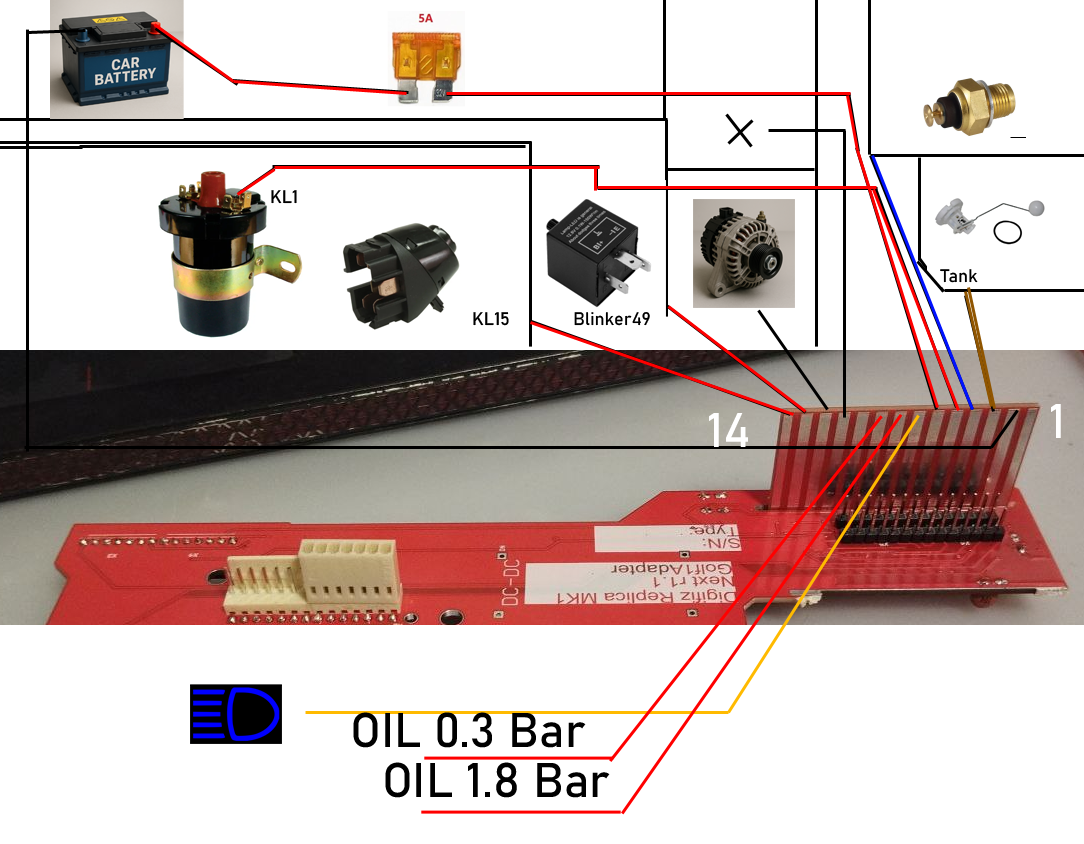
\includegraphics[width=0.75\textwidth]{digifiz_manual/image010.png}
    \caption{Схема подключения жгута для установки в Mk1.}
\end{figure}

\subsection{Сервисный разъём на печатной плате}
Третий разъём на плате повторяет цепи приборной панели; на блоках \ReplicaGenOneShort{} и \ReplicaNextShort{} пины нумеруются справа налево.
Он предоставляет сервисный интерфейс с назначениями, перечисленными в \autoref{tab:service-connector-ru}.

\begin{table}[htbp]
    \centering
    \caption{Назначение выводов сервисного разъёма.}
    \label{tab:service-connector-ru}
    {\scriptsize
    \begin{tblr}{
        colspec={Q[l,1.9cm] X[l]},
        hlines,
    }
        \textbf{Позиция} & \textbf{Назначение} \\
        1 & Выход индикатора. \\
        2 & Вход датчика скорости (SPM\_M). \\
        3 & Масса автомобиля. \\
        4 & Выход индикатора. \\
        5 & Вход оптопары левого поворотника. \\
        6 & Вход оптопары правого поворотника. \\
        7 & +12~В зажигания. \\
        8 & Специальный вход для дизеля. \\
        9 & Вход индикатора (положительный). \\
        10 & Альтернативный вход оборотов (не используется, только \ReplicaNextShort{}). \\
        11 & \ReplicaGenOneShort{}: выход индикатора (обычно не задействован); \ReplicaNextShort{}: вход тормоза (активен по массе). \\
        12 & Зарезервировано. \\
        13 & Вход индикатора неисправности двигателя. \\
        14 & Нет контакта. \\
    \end{tblr}}
\end{table}

\subsection{Разъёмы дополнительного расширения}
На основной плате установлены три дополнительных четырёхконтактных разъёма, упрощающих модернизацию жгута и сервисные работы:
\begin{itemize}
    \item \textbf{Аналоговое расширение:} отдельный вывод для подключения дополнительных аналоговых датчиков при интеграции нестандартных сенсоров.
    \item \textbf{Дублирование MFA:} повторяет стандартный разъём \textsc{MFA} для параллельного съёма сигналов бортового компьютера.
    \item \textbf{Аналоговые дубликаты:} повторяет выходы датчиков температуры масла, наружной температуры и индикатора тормоза, что позволяет подключать внешние регистраторы или блоки мониторинга.
\end{itemize}
Все три используют ответный разъём \mbox{KF2510-4p}. Он не входит в комплект поставки и при необходимости приобретается отдельно.

\begin{figure}[htbp]
    \centering
    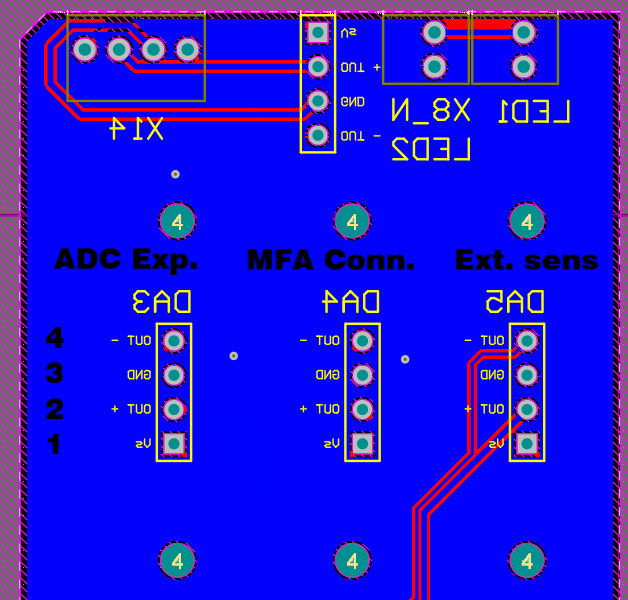
\includegraphics[width=0.6\textwidth]{digifiz_manual/ext_conn.png}
    \caption{Расположение вспомогательных разъёмов на основной плате.}
\end{figure}

\begin{table}[htbp]
    \centering
    {\small
    \begin{tblr}{
        colspec={Q[l,2.3cm] Q[c,1.3cm] X[l]},
        hlines,
        row{1} = {font=\bfseries}
    }
    Разъём & Пин & Назначение \\
    Разъём~I & 4 & Дополнительный аналоговый вход~1 \\
    Разъём~I & 3 & Масса (GND) \\
    Разъём~I & 2 & Дополнительный аналоговый вход~2 \\
    Разъём~I & 1 & Питание VCC (3V3, без предохранителя\textbf{!!!}) \\
    Разъём~II & 4 & Сброс MFA \\
    Разъём~II & 3 & Масса (GND) \\
    Разъём~II & 2 & Блок памяти MFA \\
    Разъём~II & 1 & Режим MFA \\
    Разъём~III & 4 & Выход датчика температуры масла \\
    Разъём~III & 3 & Масса (GND) \\
    Разъём~III & 2 & Выход датчика наружной температуры \\
    Разъём~III & 1 & Индикатор тормоза \\
    \end{tblr}}
    \caption{Назначение выводов вспомогательных разъёмов.}
\end{table}

\section{Встроенное ПО и комплектация}
Прошивка приборной панели опубликована по адресу:
\displayurl{https://github.com/Sgw32/DigifizReplica}
Доступны два комплекта поставки:
\begin{itemize}
    \item \textbf{\ReplicaGenOne{}:} собранная приборная панель, жгут датчиков наружной и масляной температуры, программатор USBasp и (для удалённых датчиков скорости) жгут датчика скорости.
    \item \textbf{\ReplicaNextLong{}:} собранная приборная панель и жгут электронного датчика скорости.
\end{itemize}
